\section{Further Complications}
\label{sec:complications}

[I have a note: TC1: Track local state ???]

\subsection{If Closure ($\xIF$)}
Requires indexing to resolve nondeterminism.

IF closure/case analysis: $\psi_e$

\begin{definition}[$\xIF$]
  \label{def:pomsets-if}
  Update Def.~\ref{def:pomsets-trans} to:

  If $\aPS \in \sSTOREtight[\amode]{\aLoc}{\aExp}$ then
  $(\exists\aVal:\aEvs\fun\Val)$
  $(\exists\cForm:\aEvs\fun\Formulae)$
  \begin{enumerate}
  \item[\ref{S1})] if $\cForm_\bEv\land\cForm_\aEv$ is satisfiable then $\bEv=\aEv$,
  \item[\ref{S2})] $\labelingAct(\aEv) = \DWREFP{\cVal_\aEv}{\aVal_\aEv}$,
  \item[\ref{S3})] $\labelingForm(\aEv)$ implies $\cForm_\aEv \land \aExp{=}\aVal$,
  \item[\ref{S4})] $(\forall\aEv\in\aEvs\cap\bEvs)$
    $\aTr{\bEvs}{\bForm}$ implies $\cForm_\aEv \limplies \bForm[\aExp/\aLoc]$,
  \item[\ref{S5})] 
    $\aTr{\cEvs}{\bForm}$ implies $(\!\not\exists\aEv\in\aEvs\cap\cEvs \suchthat \cForm_\aEv) \limplies \bForm[\aExp/\aLoc]$,
  \end{enumerate}

  If $\aPS \in \sLOAD[\amode]{\aReg}{\aLoc}$ then
  $(\exists\aVal:\aEvs\fun\Val)$
  $(\exists\cForm:\aEvs\fun\Formulae)$
  \begin{enumerate}
  \item[\ref{L1})] if $\cForm_\bEv\land\cForm_\aEv$ is satisfiable then $\bEv=\aEv$,
  \item[\ref{L2})] $\labelingAct(\aEv) = \DRREFP{\cVal_\aEv}{\aVal_\aEv}$,
  \item[\ref{L3})] $\labelingForm(\aEv)$ implies $\cForm_\aEv$.
  \item[\ref{L4})] $(\forall\aEv\in\aEvs\cap\bEvs)$
    $\aTr{\bEvs}{\bForm}$ implies $\cForm_\aEv \limplies \aVal_\aEv{=}\uReg{\aEv}\limplies\bForm[\uReg{\aEv}/\aReg]$, 
  \item[\ref{L5})] $(\forall\aEv\in\aEvs\setminus\cEvs)$
    $\aTr{\cEvs}{\bForm}$ implies $\cForm_\aEv \limplies (\aVal_\aEv{=}\uReg{\aEv}\lor \aLoc{=}\uReg{\aEv})\allowbreak\limplies\bForm[\uReg{\aEv}/\aReg]$,
  \item[\ref{L6})] $(\forall\bReg)$
    $\aTr{\dEvs}{\bForm}$ implies $(\!\not\exists\aEv\in\aEvs \suchthat \cForm_\aEv) \limplies \bForm[\bReg/\aReg]$. 
  \end{enumerate}  
\end{definition}

\subsection{Address Calculation ($\xADDR$)}

Do this after if closure, because problem with punning badly.

\begin{definition}[$\xADDR$]
  \label{def:pomsets-addr}
  Update Def.~\ref{def:pomsets-trans} to:
  \begin{enumerate}
  \item[\ref{S2})] $\labelingAct(\aEv) = \DW{\REF\cVal}{\aVal}$,
  \item[\ref{L2})] $\labelingAct(\aEv) = \DR{\REF{\cVal}}{\aVal}$.
  \end{enumerate}

  \begin{enumerate}
  \item[\ref{S3})] $\labelingForm(\aEv)$ implies $\cExp{=}\cVal \land \aExp{=}\aVal$,
  \item[\ref{L3})] $\labelingForm(\aEv)$ implies $\cExp{=}\cVal$.
  \end{enumerate}

  \begin{enumerate}
  \item[\ref{S4})] $(\forall\dVal)$ $\aTr{\bEvs}{\bForm}$ implies $\cExp{=}\dVal \limplies \bForm[\aExp/\REF{\dVal}]$,
  \item[\ref{S5})] $(\forall\dVal)$ $\aTr{\cEvs}{\bForm}$ implies $\cExp{=}\dVal \limplies \bForm[\aExp/\REF{\dVal}]$,
  \item[\ref{L4})] $(\forall\dVal)$ $\aTr{\bEvs}{\bForm}$ implies $\cExp{=}\dVal \limplies \aVal{=}\aReg\limplies\bForm$, 
  \item[\ref{L5})] $(\forall\dVal)$ $\aTr{\cEvs}{\bForm}$ implies $\cExp{=}\dVal \limplies (\aVal{=}\aReg\lor \REF{\dVal}{=}\aReg)\limplies\bForm$,
  \item[\ref{L6})] $(\forall\dVal)$ $\aTr{\dEvs}{\bForm}$ implies $\cExp{=}\dVal \limplies \bForm$.
  \end{enumerate}  
\end{definition}

% \subsection{Agda}
% \begin{figure*}
%   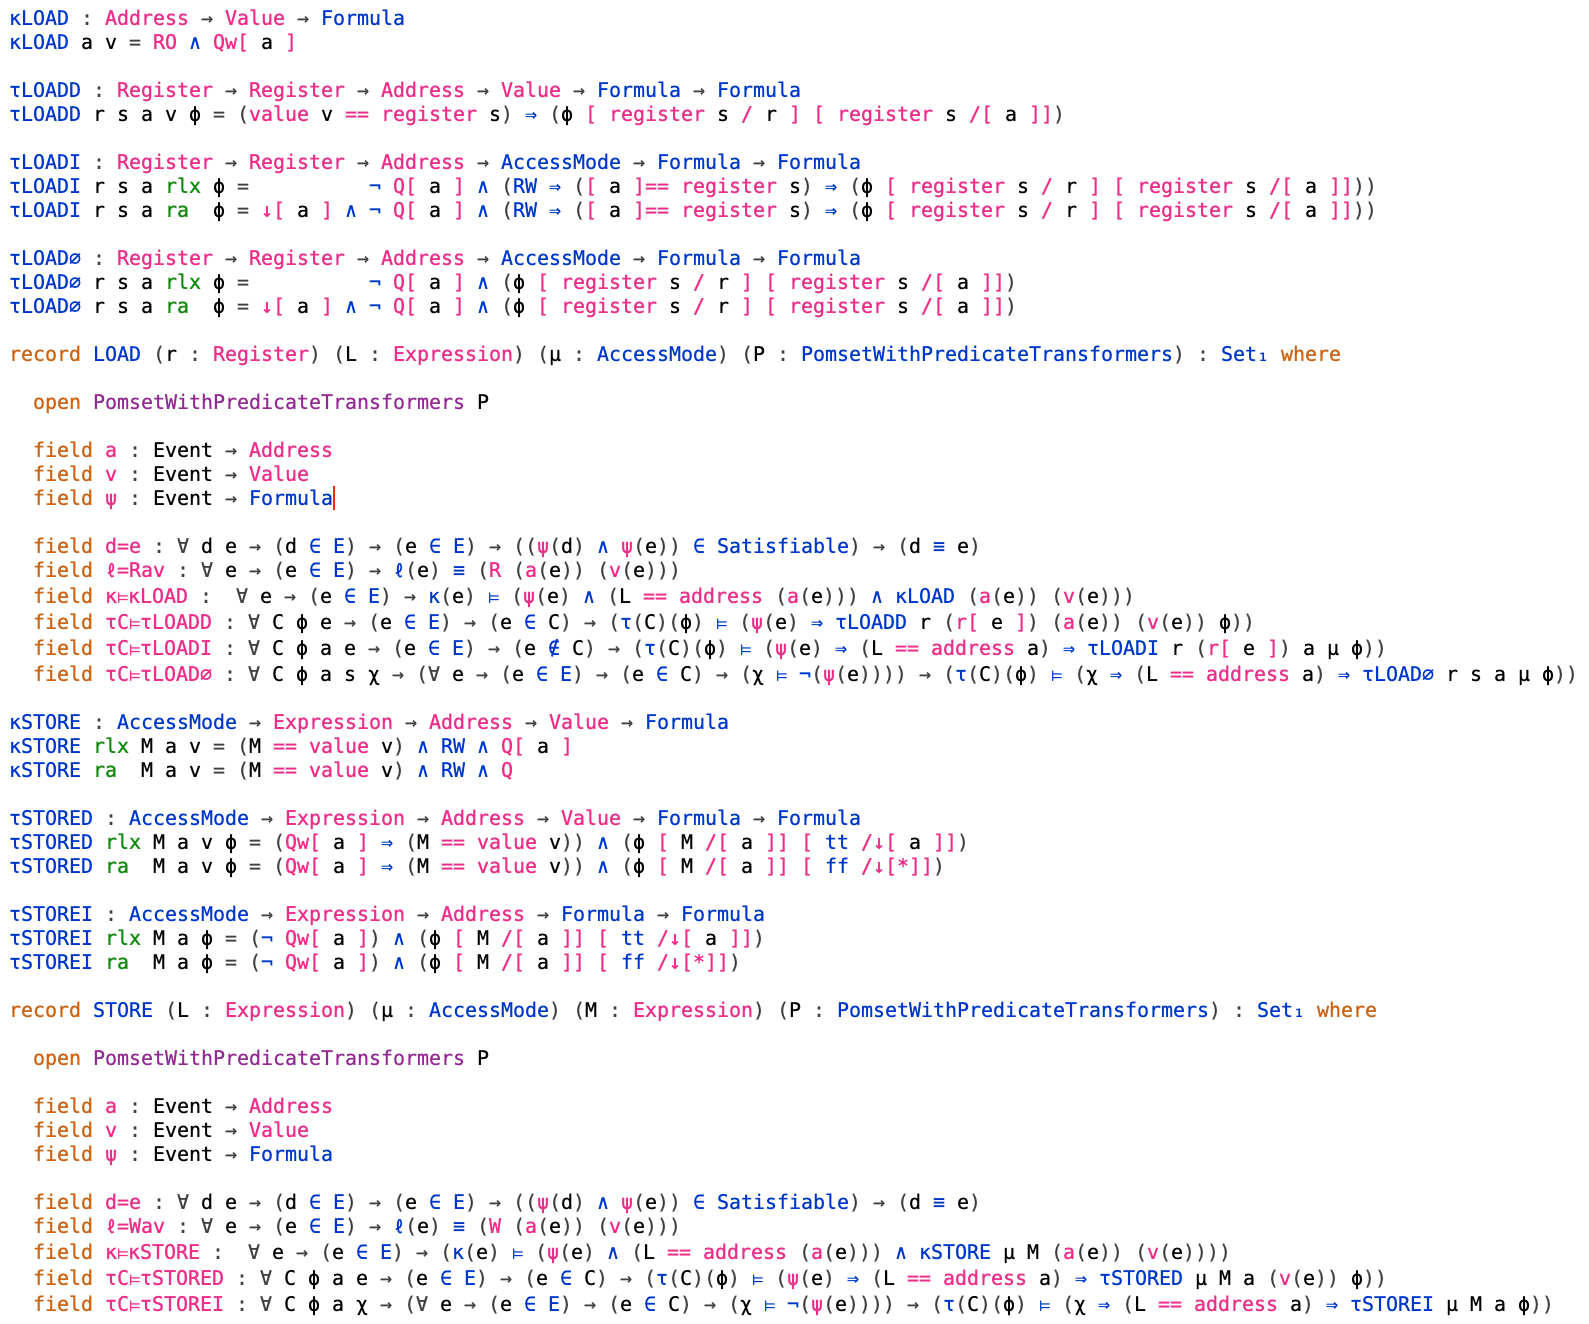
\includegraphics[width=\textwidth]{agda.png}
% \end{figure*}
